\documentclass[border=3pt]{standalone}
% Preâmbulo compartilhado pelos diagramas TikZ da aula
\usepackage[T1]{fontenc}
\usepackage[utf8]{inputenc}
\usepackage{lmodern}
\usepackage{amsmath}
\usepackage{xcolor}
\usepackage{tikz}
\usetikzlibrary{arrows.meta,angles,quotes,decorations.pathmorphing,calc,
                positioning,shapes.geometric,backgrounds,fit}

% Paleta (mesma dos SVGs originais)
\definecolor{dblue}{HTML}{2A5B8C}
\definecolor{dorange}{HTML}{B3541E}
\definecolor{dgreen}{HTML}{4A7C59}
\definecolor{dred}{HTML}{9C4B4B}
\definecolor{dcream}{HTML}{F4F1EA}
\definecolor{dshade}{HTML}{DDD7C9}

% Estilos comuns (prefixo d... para não colidir com chaves internas do pgf)
\tikzset{
  >={Stealth[length=2mm]},
  dguide/.style={gray!55, dashed, line width=0.4pt},
  daxis/.style={gray!60, line width=0.7pt, ->},
  dbody/.style={fill=black!3, draw=black!80, line width=1pt},
  dacc/.style={draw=dblue, line width=1pt},
  dlbl/.style={black!55, font=\small},
  dsub/.style={black!45, font=\footnotesize},
  dstate/.style={circle, draw=black!80, fill=dcream, line width=1pt,
                 minimum size=17mm, font=\large, inner sep=1pt},
  dobs/.style={circle, draw=black!80, fill=dshade, line width=1pt,
               minimum size=14mm, font=\large, inner sep=1pt},
  dbox/.style={rounded corners=2pt, draw=black!80, fill=dcream, line width=1pt,
               align=center, inner sep=6pt},
  dtrans/.style={->, dblue, line width=1pt},
  dmeas/.style={->, dorange, line width=1pt},
}

\begin{document}
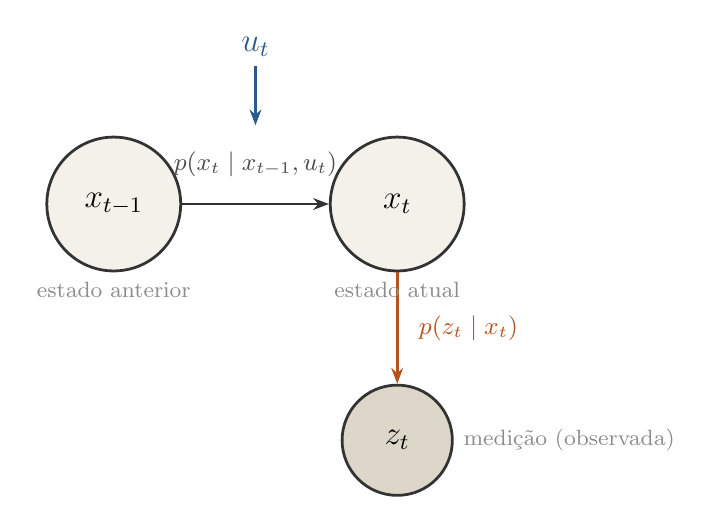
\begin{tikzpicture}[x=1cm,y=1cm]

  \node[dstate] (xp) at (0,0)   {$x_{t-1}$};
  \node[dstate] (xt) at (3.6,0) {$x_t$};
  \node[dobs]   (zt) at (3.6,-3){$z_t$};

  % entrada de controle
  \node[dblue, font=\large] (u) at (1.8,2) {$u_t$};
  \draw[dtrans] (u) -- (1.8,1.0);

  % transição
  \draw[->, black!80, line width=1pt] (xp) -- (xt)
        node[midway, above=6pt, black!70, font=\small] {$p(x_t \mid x_{t-1}, u_t)$};

  % medição
  \draw[dmeas] (xt) -- (zt)
        node[midway, right=4pt, dorange, font=\small] {$p(z_t \mid x_t)$};

  \node[dsub] at (xp.south) [below] {estado anterior};
  \node[dsub] at (xt.south) [below] {estado atual};
  \node[dsub] at (zt.east)  [right] {medição (observada)};

\end{tikzpicture}
\end{document}
